{\color{ggreen}\subsection{Metodo di Regolarizzazione di Tikhonov}}
Per ridurre gli effetti del rumore nella ricostruzione si può aggiungere al problema precendente un 
termine di regolarizzazione di Tikhonov. 

Si considera quindi il seguente problema di ottimizzazione:

Al posto di risolvere direttamente il sistema lineare (se il sistema è quadrato) o di minimizzare la norma 2 del residuo 
$||Ax_\epsilon -b_\epsilon||_2^2$ (se il sistema è rettangolare), 

si aggiunge un termine "rilassatore" al problema naive precedente e lo si minimizza, ad esempio 
\[||Ax_\epsilon-b_\epsilon||_2^2+\gamma_\epsilon||x_\epsilon||_2^2\] 
{\centering $Ax_\epsilon = b_\epsilon$ con $b_\epsilon = b+\epsilon$}

\begin{figure}[H]
    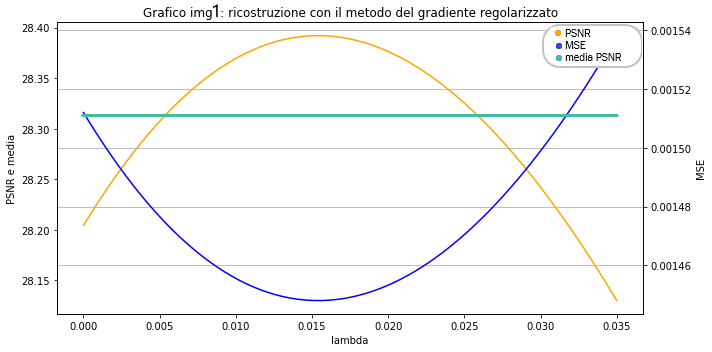
\includegraphics[width=0.5\textwidth]{IMMAGINI_RELAZIONE/grafico1Tik.png}
    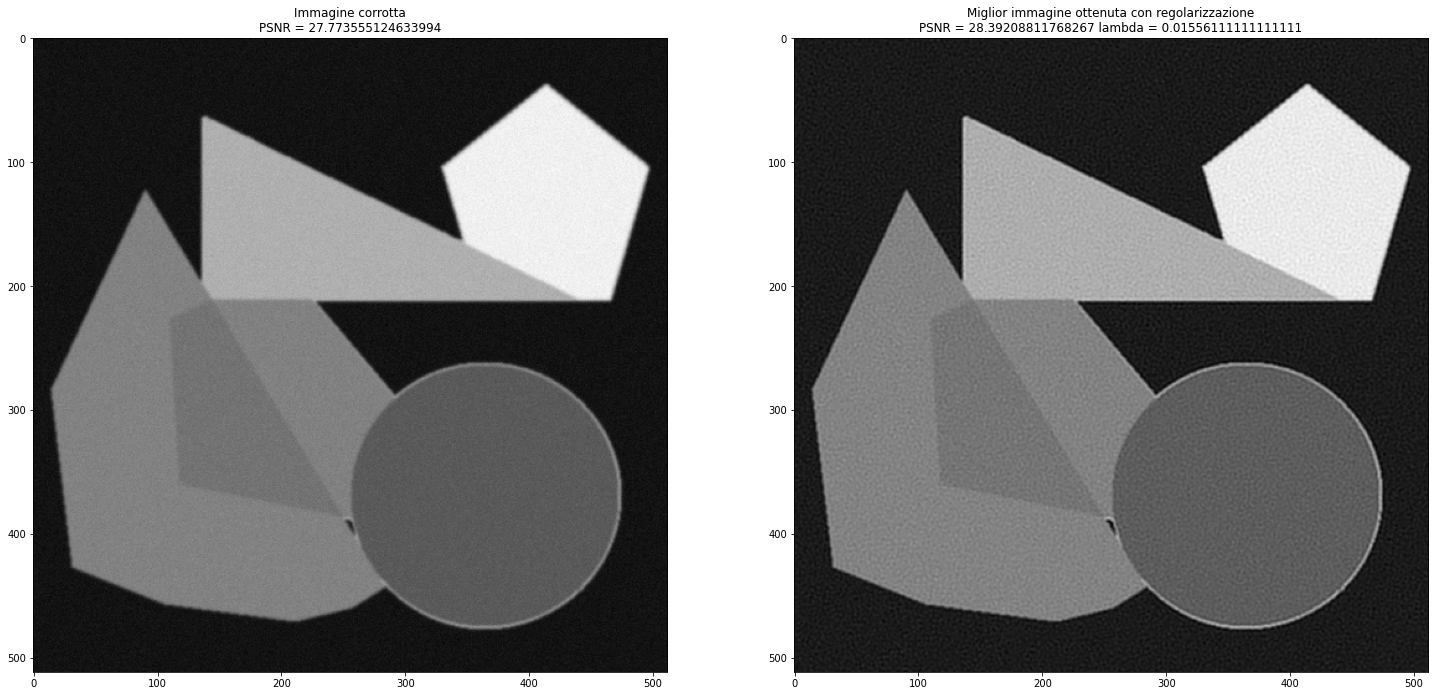
\includegraphics[width=0.5\textwidth]{IMMAGINI_RELAZIONE/ricostruzione1Tik.png}
    \caption{Ricostruzione immagine geometrica img1.png}

    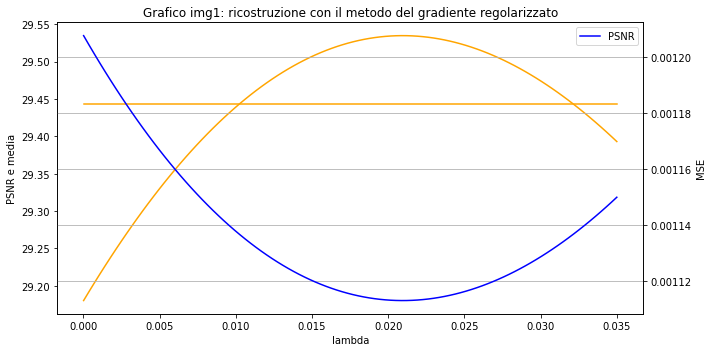
\includegraphics[width=0.5\textwidth]{IMMAGINI_RELAZIONE/grafico2Tik.png}
    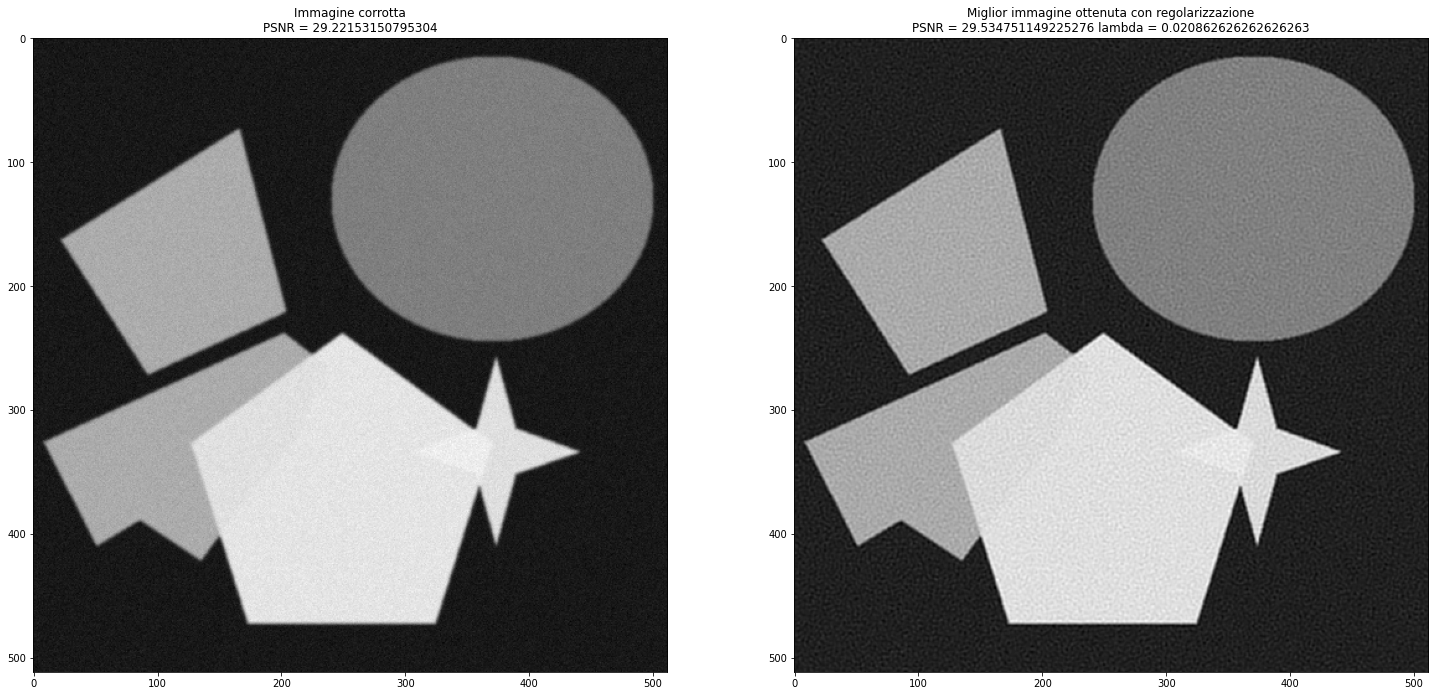
\includegraphics[width=0.5\textwidth]{IMMAGINI_RELAZIONE/ricostruzione2Tik.png}
    \caption{Ricostruzione immagine geometrica img2.png}

    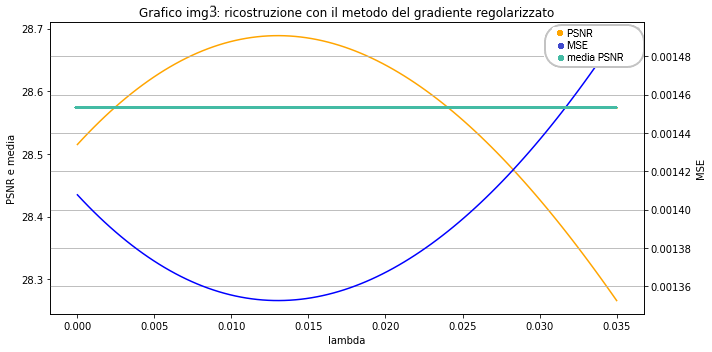
\includegraphics[width=0.5\textwidth]{IMMAGINI_RELAZIONE/grafico3Tik.png}
    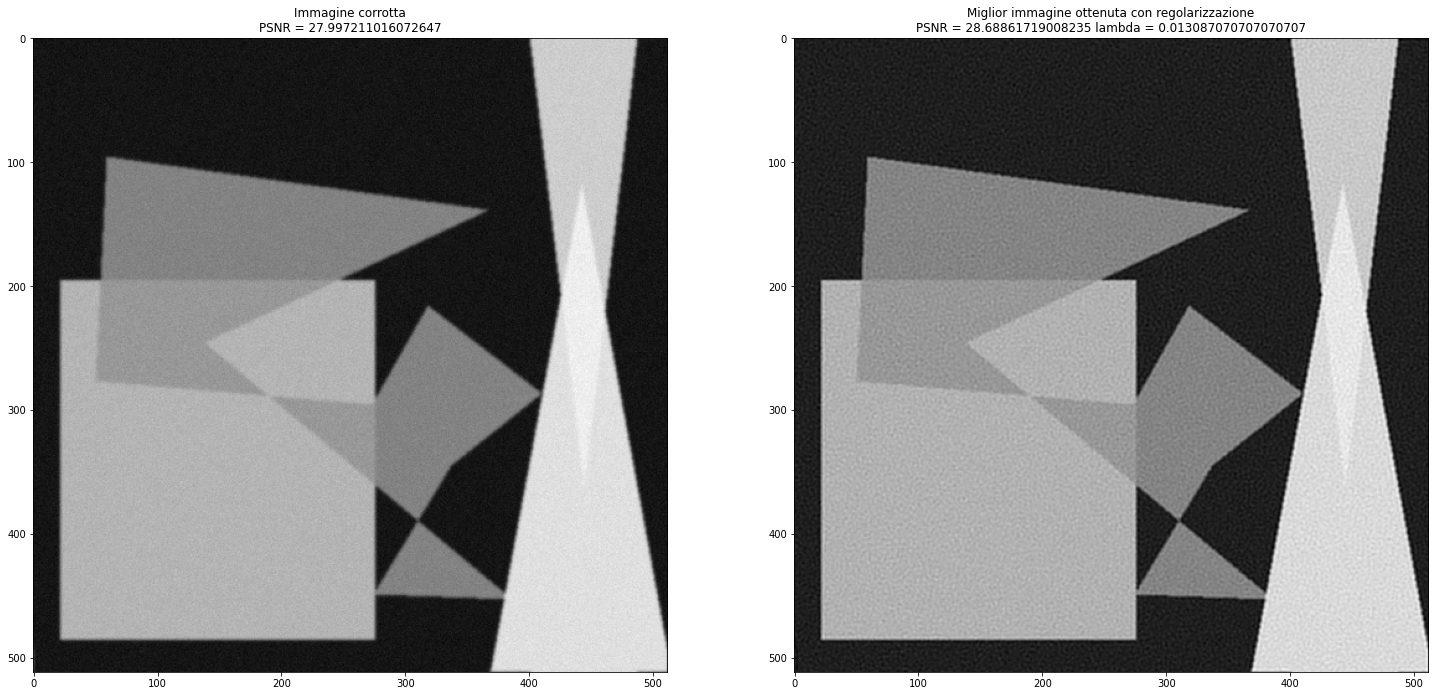
\includegraphics[width=0.5\textwidth]{IMMAGINI_RELAZIONE/ricostruzione3Tik.png}
    \caption{Ricostruzione immagine geometrica img3.png}
\end{figure}

\begin{figure}[H]
    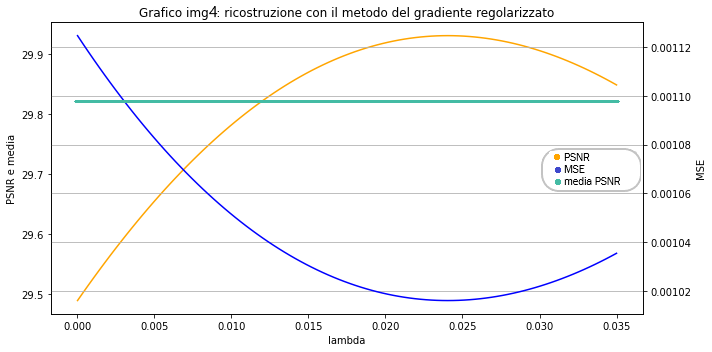
\includegraphics[width=0.5\textwidth]{IMMAGINI_RELAZIONE/grafico4Tik.png}
    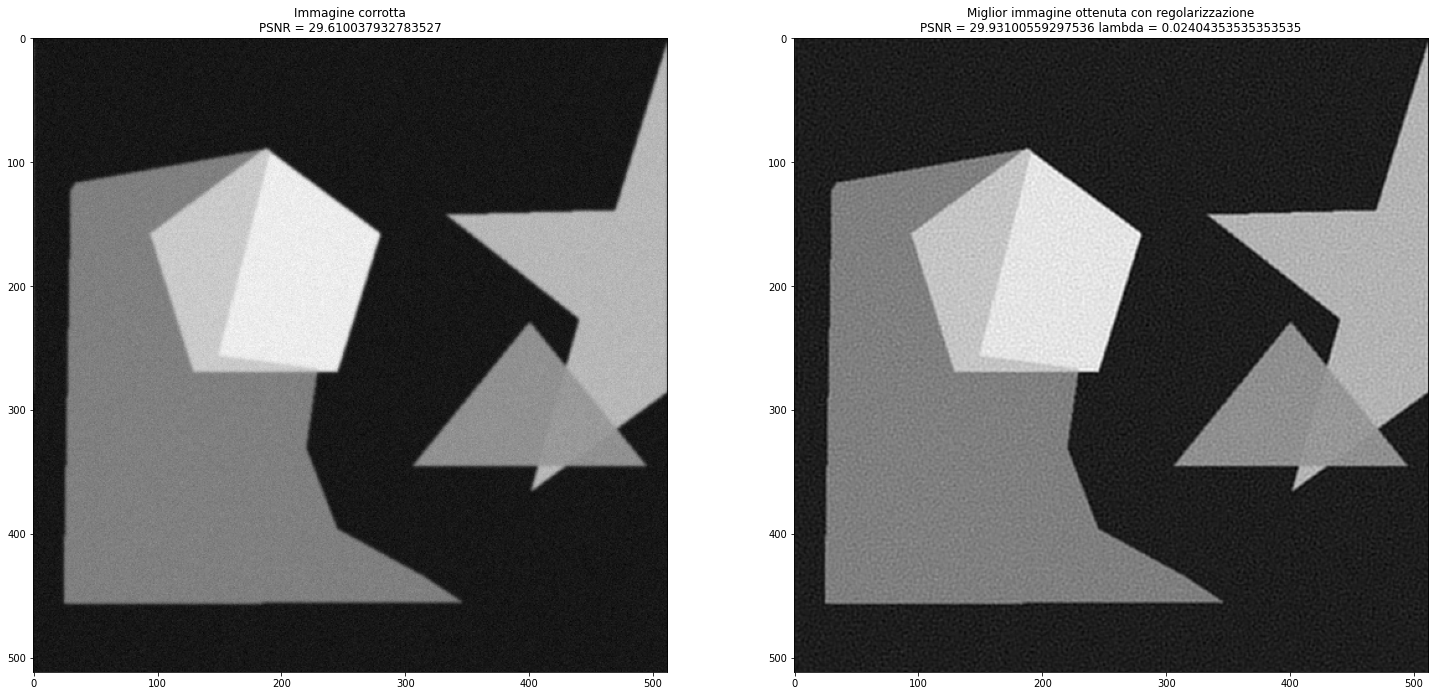
\includegraphics[width=0.5\textwidth]{IMMAGINI_RELAZIONE/ricostruzione4Tik.png}
    \caption{Ricostruzione immagine geometrica img4.png}

    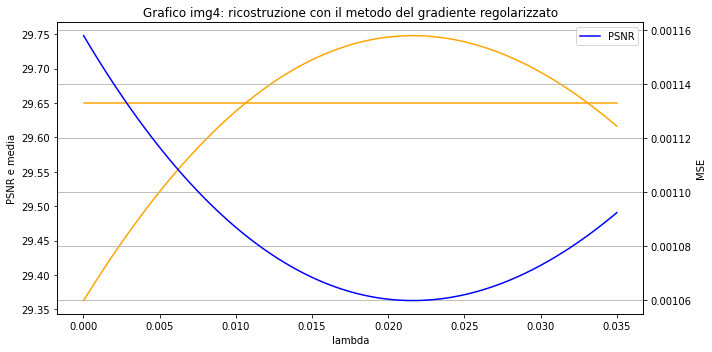
\includegraphics[width=0.5\textwidth]{IMMAGINI_RELAZIONE/grafico5Tik.png}
    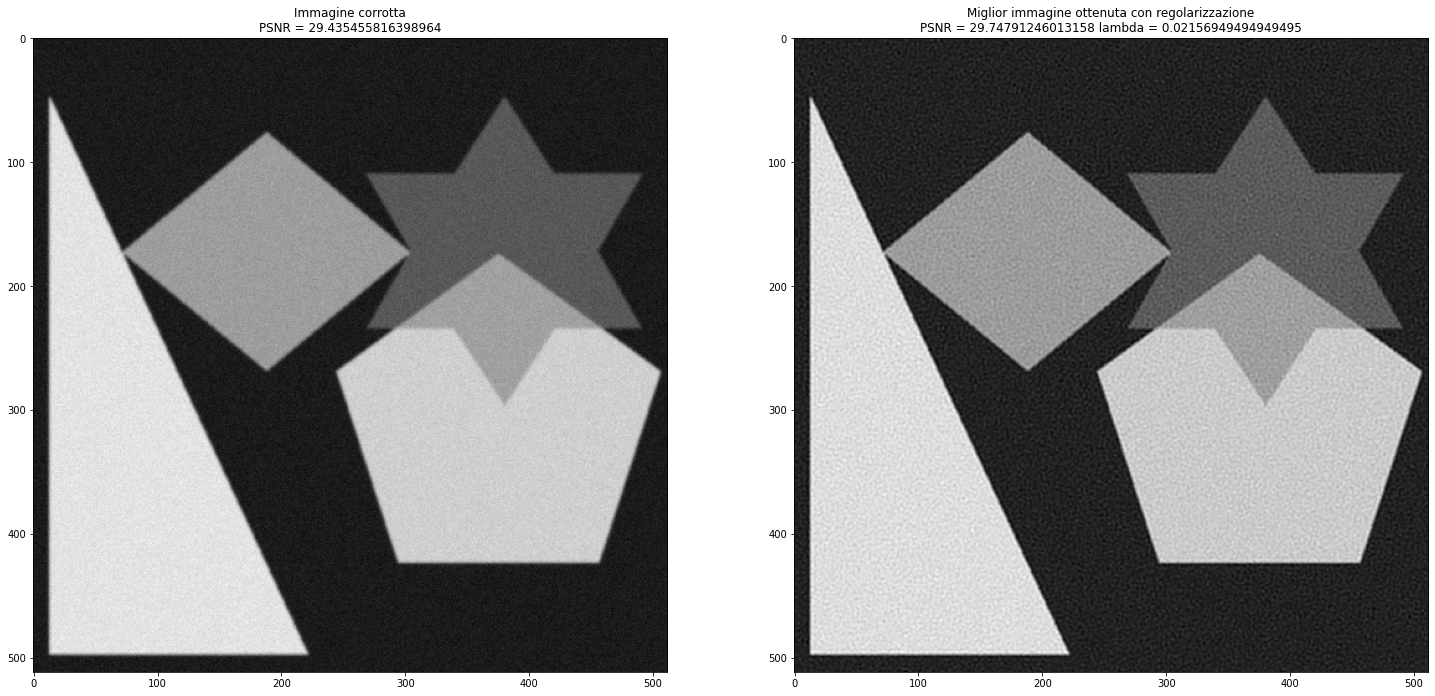
\includegraphics[width=0.5\textwidth]{IMMAGINI_RELAZIONE/ricostruzione5Tik.png}
    \caption{Ricostruzione immagine geometrica img5.png}

    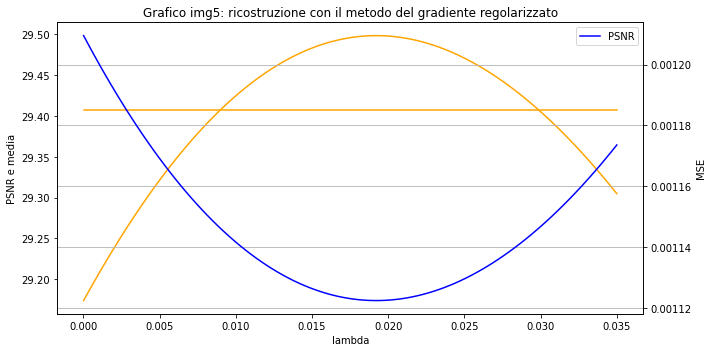
\includegraphics[width=0.5\textwidth]{IMMAGINI_RELAZIONE/grafico6Tik.png}
    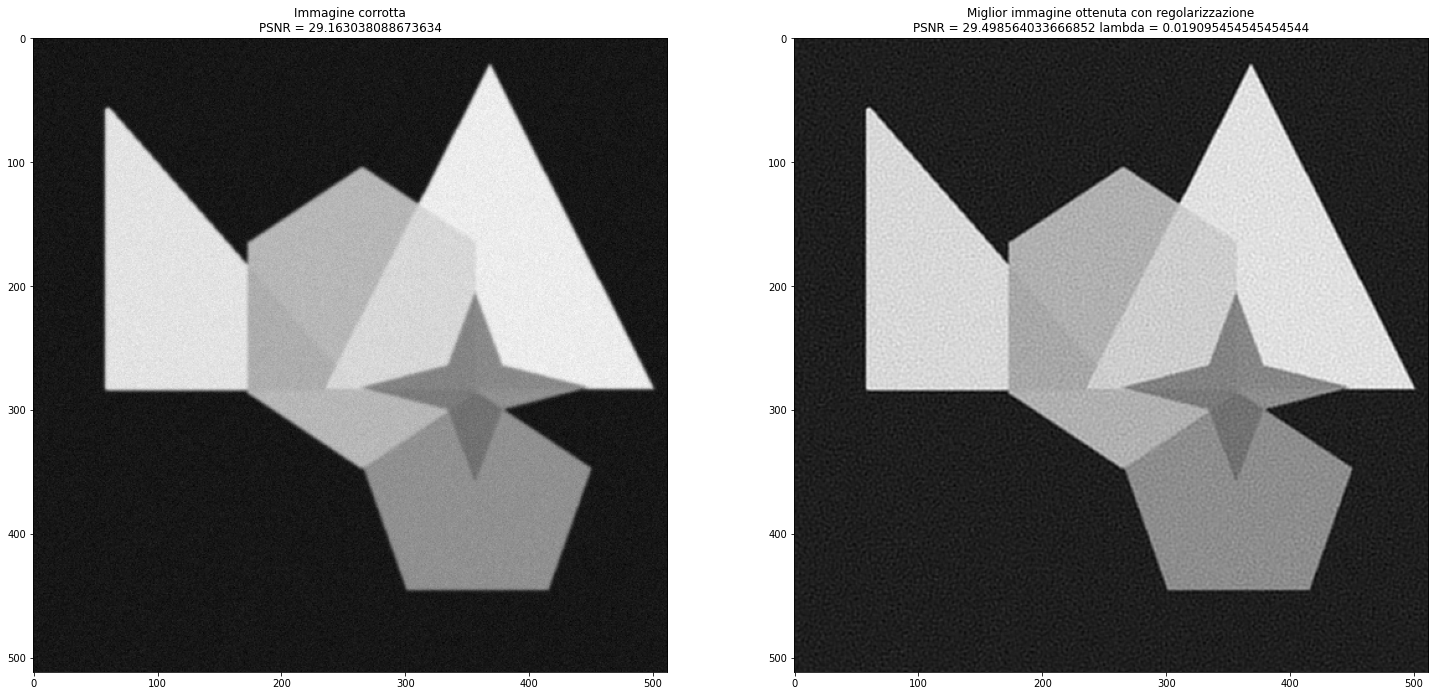
\includegraphics[width=0.5\textwidth]{IMMAGINI_RELAZIONE/ricostruzione6Tik.png}
    \caption{Ricostruzione immagine geometrica img6.png}

    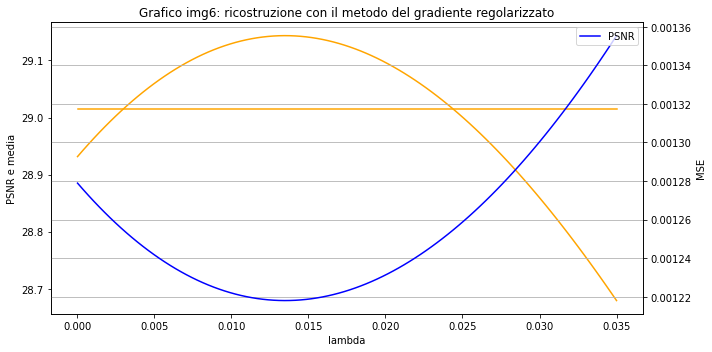
\includegraphics[width=0.5\textwidth]{IMMAGINI_RELAZIONE/grafico7Tik.png}
    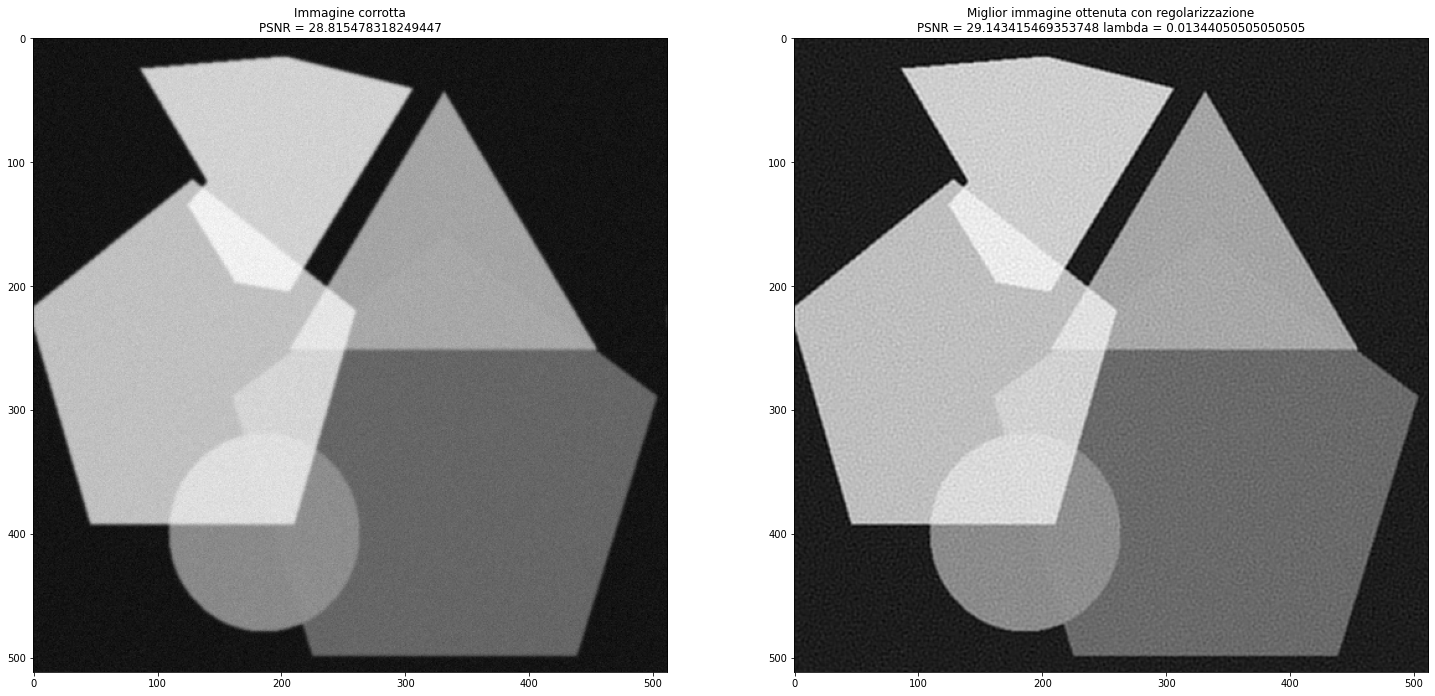
\includegraphics[width=0.5\textwidth]{IMMAGINI_RELAZIONE/ricostruzione7Tik.png}
    \caption{Ricostruzione immagine geometrica img7.png}

    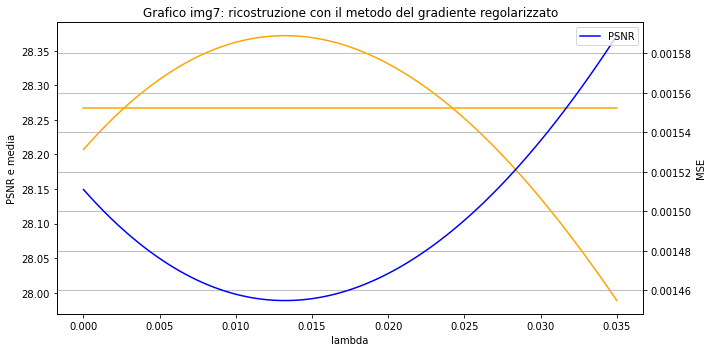
\includegraphics[width=0.5\textwidth]{IMMAGINI_RELAZIONE/grafico8Tik.png}
    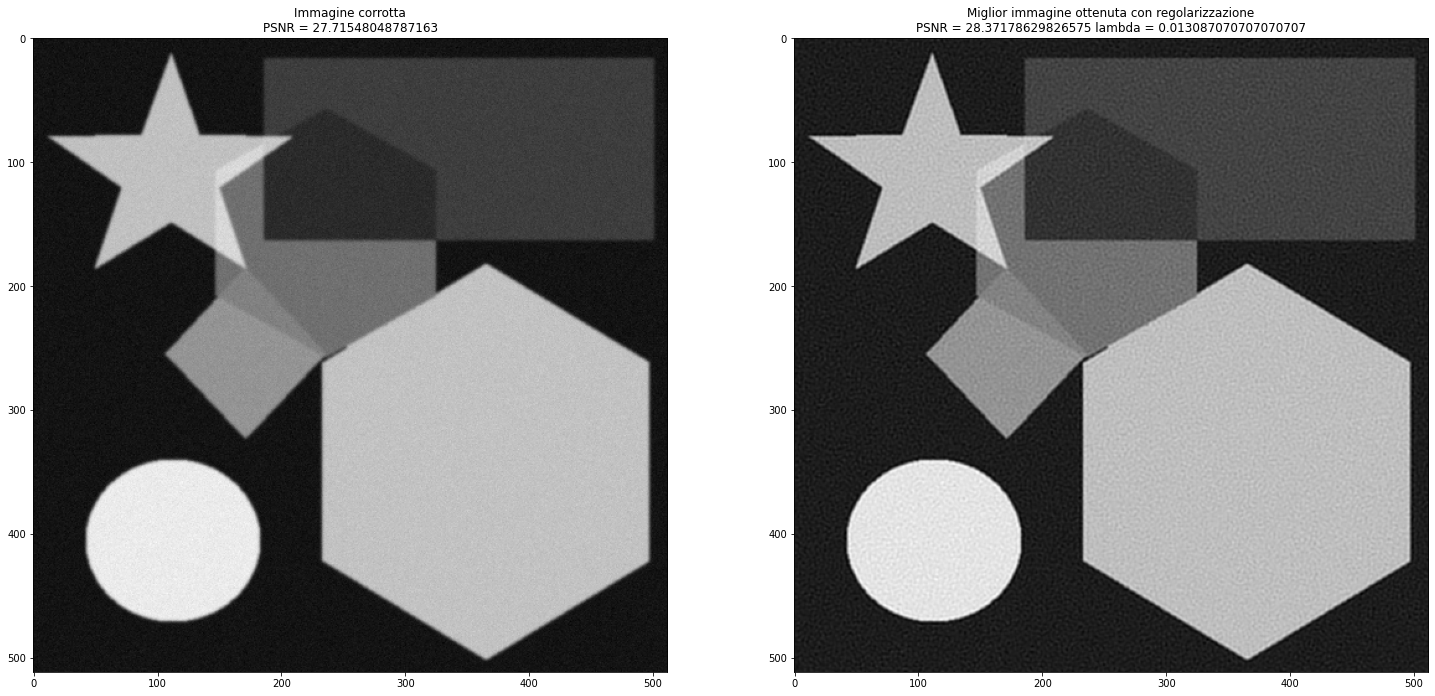
\includegraphics[width=0.5\textwidth]{IMMAGINI_RELAZIONE/ricostruzione8Tik.png}
    \caption{Ricostruzione immagine geometrica img8.png}
\end{figure}

\begin{figure}[H]
    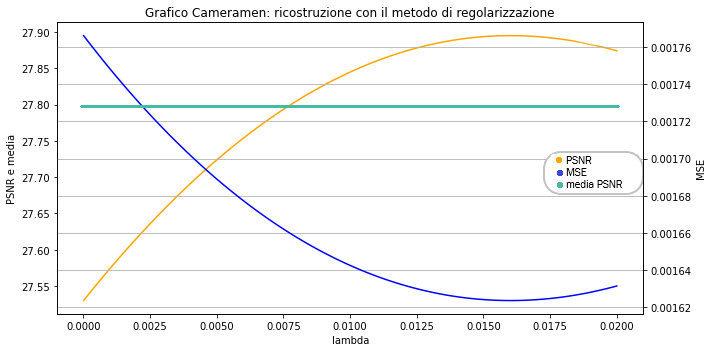
\includegraphics[width=0.5\textwidth]{IMMAGINI_RELAZIONE/graficoCameramanTik.png}
    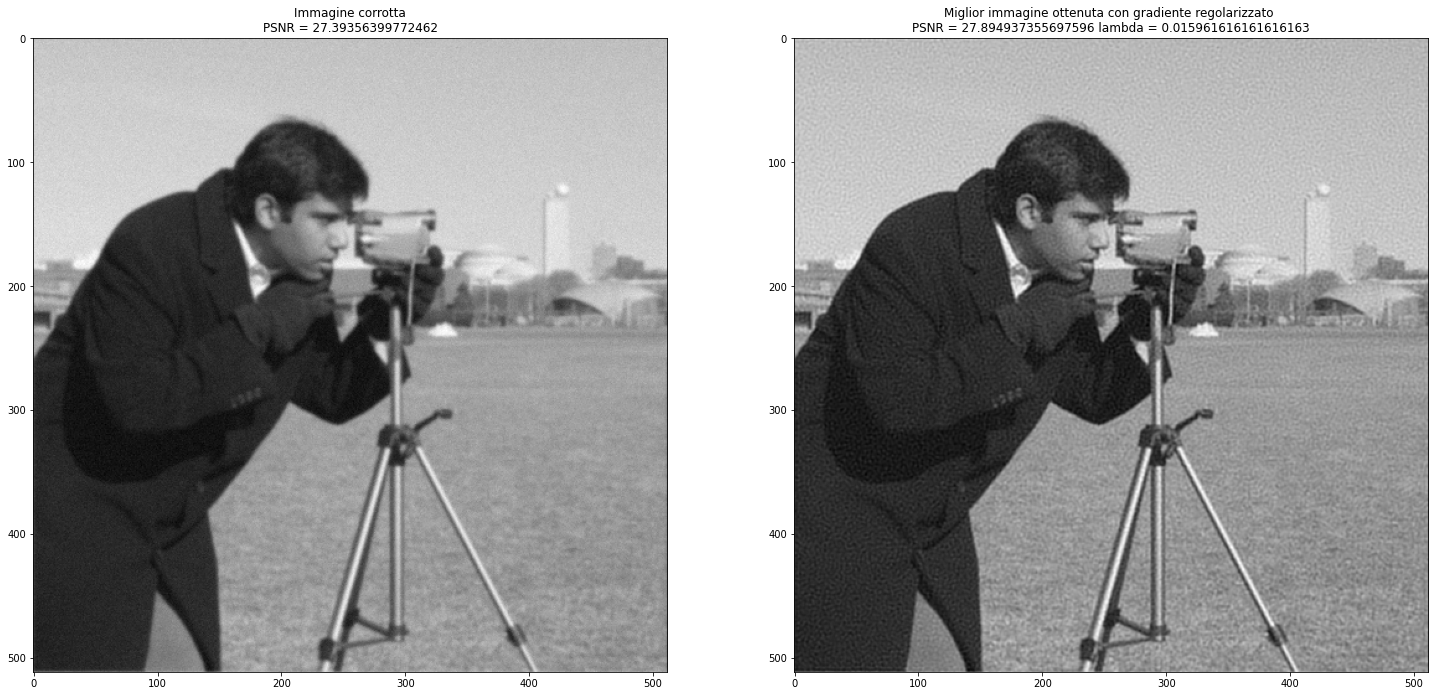
\includegraphics[width=0.5\textwidth]{IMMAGINI_RELAZIONE/ricostruzioneCameramanTik.png}
    \caption{Ricostruzione immagine fotografica data.camera()}

    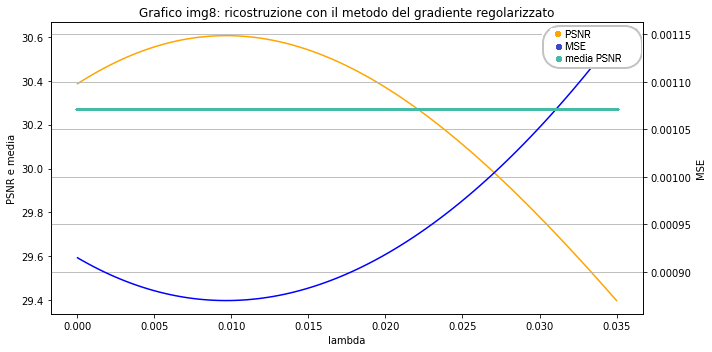
\includegraphics[width=0.5\textwidth]{IMMAGINI_RELAZIONE/graficoPugileTik.png}
    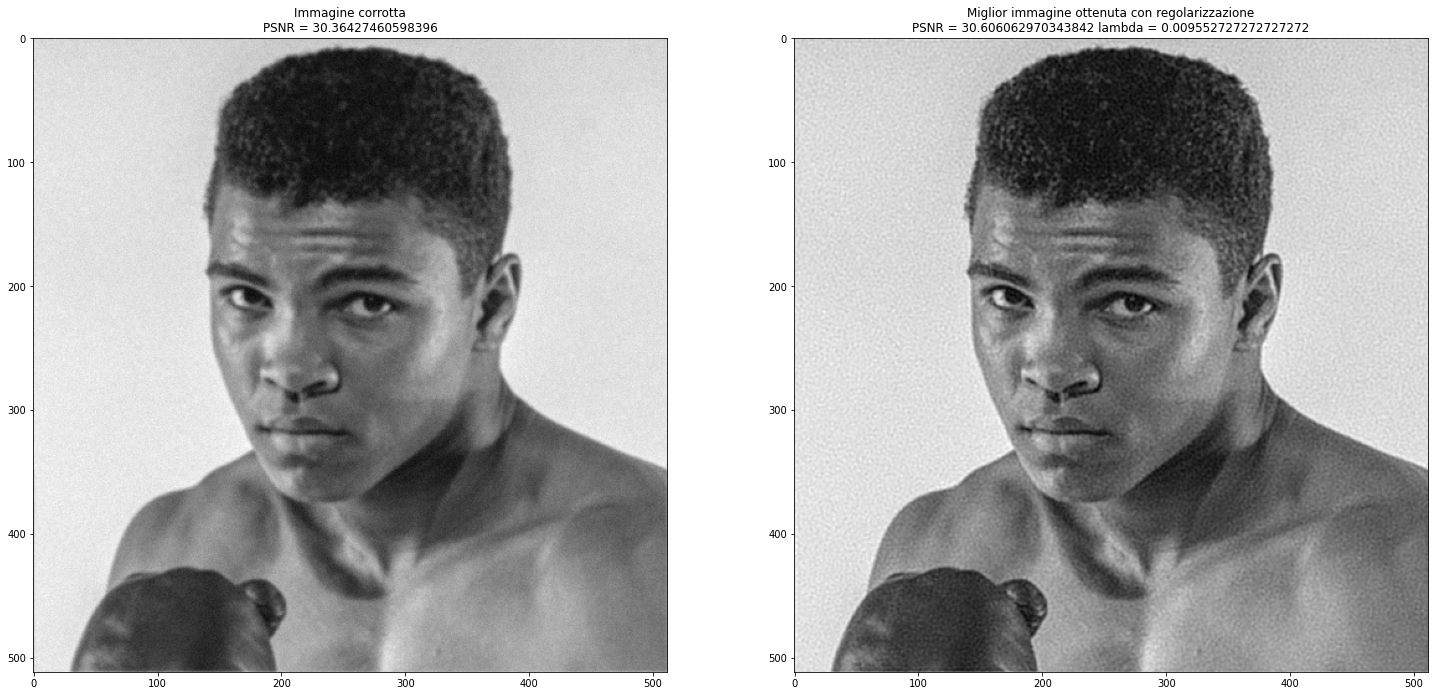
\includegraphics[width=0.5\textwidth]{IMMAGINI_RELAZIONE/ricostruzionePugileTik.png}
    \caption{Ricostruzione immagine fotografica pugile.png}
\end{figure}